\chapter{Implementación, Pruebas y Resultados}
\label{chap:implementacion}

\section{Requisitos de Implementación}
Para llevar a cabo el desarrollo y despliegue del Asistente Virtual Inteligente, se establecieron diversos requisitos técnicos tanto a nivel de hardware como de software. Esto garantiza que la arquitectura distribuida del prototipo funcione sin cuellos de botella y de manera orquestada.

\subsection{Requisitos de Hardware}
El sistema fue implementado y probado en un entorno local con las siguientes especificaciones recomendadas para soportar la carga asíncrona y la inferencia generativa:
\begin{itemize}
    \item \textbf{Procesador (CPU):} Intel Core i7 de 12.ª generación (o superior), necesario para manejar la concurrencia de WebSockets y FastAPI.
    \item \textbf{Memoria RAM:} 32 GB, requeridos para cargar el entorno virtual de Python, ChromaDB y los modelos ligeros en memoria.
    \item \textbf{Tarjeta Gráfica (GPU):} NVIDIA RTX 3060 de 12GB VRAM. Fundamental para la generación acelerada de respuestas si se usan modelos LLM cuantizados locales.
    \item \textbf{Periféricos del Cliente:} Cámara web estándar (resolución mínima 640x480) y micrófono integrado para capturar las intenciones del usuario.
\end{itemize}

\subsection{Requisitos de Software y Tecnologías}
El entorno de desarrollo requiere la instalación y configuración de múltiples herramientas tecnológicas, resumidas a continuación:

\begin{table}[htbp]
  \caption{Software y herramientas requeridas para la implementación.}
  \label{tab:requisitos_software}
  \centering
  \renewcommand{\arraystretch}{1.25}
  \begin{tabular}{|p{4cm}|p{11cm}|}
    \hline
    \rowcolor[HTML]{EFEFEF}
    \textbf{Herramienta / Framework} & \textbf{Propósito y Configuración} \\ \hline
    \textbf{Python 3.10+} & Lenguaje principal del Backend. Requiere configuración de un entorno virtual (venv) e instalación de dependencias vía \texttt{requirements.txt}. \\ \hline
    \textbf{FastAPI y Uvicorn} & Framework para construir la API Gateway y manejar conexiones asíncronas y WebSockets. \\ \hline
    \textbf{ChromaDB} & Base de datos vectorial embebida. Se debe configurar para persistencia local en disco. \\ \hline
    \textbf{SentenceTransformers} & Librería para vectorización matemática (Modelo \texttt{paraphrase-\-multilingual-\-MiniLM-\-L12-\-v2}). \\ \hline
    \textbf{HTML, CSS, JS (Vite/Three.js)} & Capa Frontend. Requiere configuración para renderizar gráficos WebGL y capturar media del usuario. \\ \hline
    \textbf{Docker y Docker Compose} & Opcional para el despliegue de contenedores aislados. Requiere escritura de un \texttt{Dockerfile}. \\ \hline
  \end{tabular}
\end{table}

\begin{table}[H]
  \caption{Matriz Comparativa: Proceso Manual vs. Asistente Virtual.}
  \label{tab:matriz_comparativa}
  \centering
  
  
  \renewcommand{\arraystretch}{1.2}
  \begin{tabular}{|p{0.25\textwidth}|p{0.33\textwidth}|p{0.33\textwidth}|}
    \hline
    \rowcolor[HTML]{EFEFEF}
    \textbf{Criterio} & \textbf{Antes (Manual/SGA)} & \textbf{Después (Protopipo de IA)} \\ \hline
    \textbf{Modo de Interacción} & Navegación manual por menús. & Conversacional (Voz natural). \\ \hline
    \textbf{Formato de Respuesta} & Archivos estáticos (PDF). & Respuestas orales y visuales exactas. \\ \hline
    \textbf{Esfuerzo del Usuario} & Alto (búsqueda y lectura exhaustiva). & Bajo (solo requiere preguntar). \\ \hline
    \textbf{Soporte a Dudas} & Acudir a secretaría (demorado). & Capacidad técnica de ofrecer consultas fuera del horario administrativo, condicionada a la disponibilidad de infraestructura. \\ \hline
  \end{tabular}
\end{table}

\section{Proceso de Implementación}
El proceso de implementación siguió un enfoque iterativo, comenzando desde la configuración de la base de datos y culminando con el ensamblaje de la interfaz de usuario en el frontend. A continuación, se detallan los pasos lógicos.

\subsection{Paso 1: Configuración a nivel de Base de Datos Vectorial}
El primer paso consistió en la inicialización y población de \textbf{ChromaDB}. Se desarrolló el script \texttt{rag\_manager.py} que toma los reglamentos y mallas curriculares (archivos PDF), los extrae y divide en fragmentos semánticos (\textit{chunks}). Posteriormente, utilizando \texttt{SentenceTransformers}, cada bloque de texto se convierte en un arreglo numérico y se inserta en una colección persistente llamada \texttt{carrera\_ti\_indoamerica\_collection}. Este proceso debe ejecutarse y completarse antes de levantar el servidor, pues el motor de inteligencia artificial depende de este conocimiento previo.

Para ilustrar la estructuración de la base de datos vectorial, a continuación se presenta un ejemplo representativo de cómo se almacena un registro en ChromaDB (formato JSON):

\begin{verbatim}
{
  "id": "Reglamento_Academico_chunk_42",
  "document": "Art. 15.- Las modalidades de titulacion incluyen...",
  "embedding": [0.0124, -0.0453, 0.8921, ...],
  "metadata": {
    "source": "Reglamento_Titulacion_2024.pdf",
    "page": 12,
    "tipo_documento": "Normativa Institucional"
  }
}
\end{verbatim}

Esta estructura de almacenamiento separada se diseñó estratégicamente por dos razones. Primero, el modelo de \textit{embedding} procesa exclusivamente el campo \texttt{document} (contenido puro) para calcular la similitud semántica con la consulta del usuario, evitando que palabras de control o datos referenciales modifiquen la pureza del vector matemático. Segundo, el diccionario \texttt{metadata} permite aislar los datos de origen; esto habilita al sistema para aplicar filtros cruzados preventivos antes de buscar (\textit{metadata filtering}) y permite que el Asistente Virtual cite de forma transparente al usuario la página exacta y el nombre del documento oficial de donde extrajo la respuesta.

\begin{figure}[htbp]
  \centering
  \includegraphics[width=0.9\textwidth]{Logos/diagrama_bd_chroma.png}
  \caption{Estructura lógica y proceso de vectorización en la base de datos ChromaDB.}
  \label{fig:bd_chroma}
\end{figure}

\begin{figure}[htbp]
  \centering
  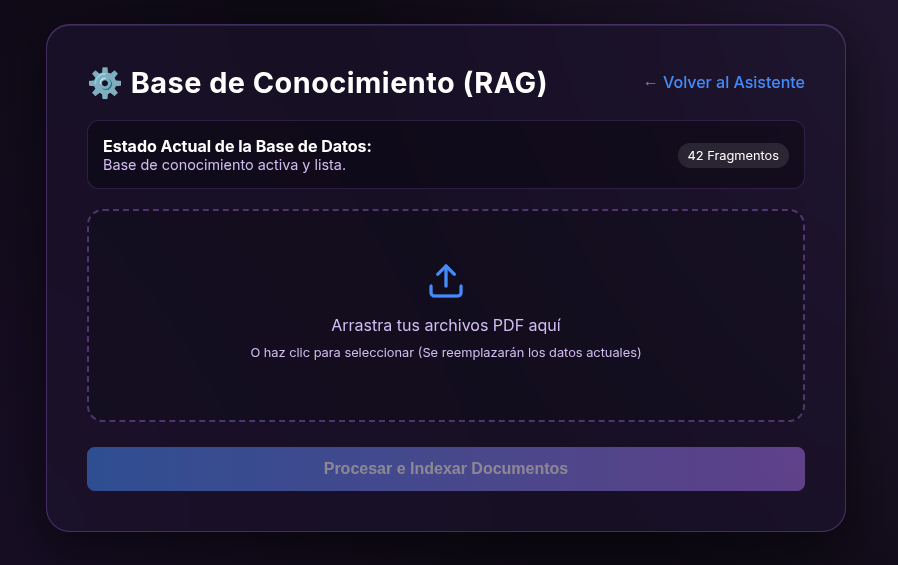
\includegraphics[width=0.9\textwidth]{Logos/Seccion_AdminRAG.png}
  \caption{Panel de Administración del RAG para actualizar mallas curriculares.}
  \label{img:admin_rag}
  \elaboradopor{Estudiante}
  \fuente{Captura de pantalla del sistema}
\end{figure}

\subsection{Paso 2: Construcción del Servidor Backend (FastAPI)}
Una vez establecida la base de datos, se programó el orquestador principal: el archivo \texttt{api.py}. En este nivel de aplicación se configuraron las rutas (endpoints) RESTful y las conexiones WebSockets. El servidor se encarga de:
1. Recibir fotogramas ligeros vía WebSockets y calcular el área del \textit{bounding box} del rostro ($W_{box} \times H_{box}$) para determinar presencia activa, de acuerdo al siguiente modelo lógico:

\begin{equation}
\label{eq:presence}
Estado = 
\begin{cases} 
Activo, & \text{si } (W_{box} \times H_{box}) > \tau_{pixeles} \\
Reposo, & \text{de lo contrario}
\end{cases}
\end{equation}
\addeqtolist{Cálculo lógico para detección de presencia del usuario vía WebSockets}
2. Recibir audios en formato WebM, enviarlos a Groq API (Whisper-v3) para transcripción ultrarrápida.
3. Orquestar la consulta a ChromaDB usando la similitud del coseno.
4. Conectar con el LLM para formular la respuesta y luego con ElevenLabs para el proceso de Text-to-Speech (TTS).

\begin{figure}[htbp]
\centering
\begin{tikzpicture}[
    scale=0.85, transform shape,
    box/.style={draw, rounded corners, fill=blue!10, minimum width=3cm, minimum height=1cm, align=center, text width=2.8cm},
    arrow/.style={->, >=stealth, thick}
]
% Nodes
\node[box] (mic) {Cliente (Micrófono)};
\node[box, right=3.5cm of mic] (fastapi) {FastAPI (Backend)};
\node[box, fill=green!10, above right=0.8cm and 1.5cm of fastapi] (groq) {API Groq (Whisper-v3)};
\node[box, fill=orange!10, below right=0.8cm and 1.5cm of fastapi] (eleven) {ElevenLabs (TTS Streaming)};
\node[box, right=2cm of groq] (llm) {Motor LLM / RAG};
% Arrows
\draw[arrow] (mic) to[bend left=15] node[above] {\small Audio .webm} (fastapi);
\draw[arrow] (fastapi) |- node[above, near start] {\small Delegar Audio} (groq);
\draw[arrow] (groq) -- node[above] {\small Texto} (llm);
\draw[arrow] (llm) -- node[right] {\small Respuesta Textual} (eleven);
\draw[arrow] (eleven) -| node[below, near end] {\small Audio (Chunks)} (fastapi);
\draw[arrow] (fastapi) to[bend left=15] node[below] {\small Audio Frontend} (mic);
\end{tikzpicture}
\caption{Diagrama de delegación y procesamiento de voz asíncrono en el backend.}
\label{fig:flujo_voz}
\end{figure}

\subsection{Paso 3: Desarrollo de la Capa de Cliente (Frontend)}
A nivel de frontend, se diseñó la interfaz dual que permite a los usuarios interactuar. Se integró Three.js para renderizar un avatar 3D (formato VRM) provisto por Ready Player Me. La aplicación cliente captura los \textit{streams} de audio y video utilizando \texttt{navigator.mediaDevices} y los remite al servidor. Además, recibe los \textit{chunks} de audio de respuesta e interpreta los fonemas (visemas) para sincronizar el movimiento de la boca del avatar, generando una presencia empática.

\begin{figure}[htbp]
\centering
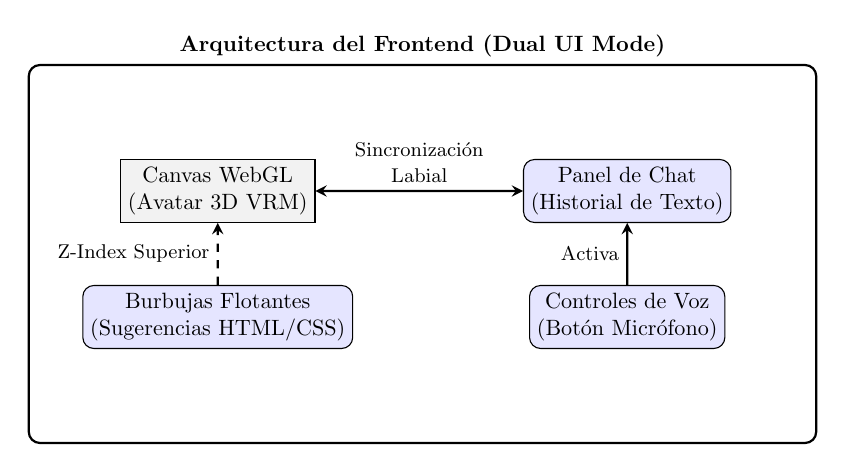
\begin{tikzpicture}[
    scale=0.8, transform shape,
    component/.style={draw, fill=gray!10, rectangle, minimum width=3cm, minimum height=1cm, align=center},
    ui/.style={draw, fill=blue!10, rectangle, minimum width=3cm, minimum height=1cm, align=center, rounded corners},
    arrow/.style={->, >=stealth, thick}
]
% Background box representing the browser
\draw[fill=white, thick, rounded corners] (-1,-1) rectangle (11.5,5);
\node[above] at (5.25,5) {\textbf{Arquitectura del Frontend (Dual UI Mode)}};
% Components
\node[component] (webgl) at (2, 3) {Canvas WebGL\\(Avatar 3D VRM)};
\node[ui] (bubbles) at (2, 1) {Burbujas Flotantes\\(Sugerencias HTML/CSS)};
\node[ui] (chat) at (8.5, 3) {Panel de Chat\\(Historial de Texto)};
\node[ui] (mic) at (8.5, 1) {Controles de Voz\\(Botón Micrófono)};
% Arrows
\draw[arrow, dashed] (bubbles) -- node[left] {\small Z-Index Superior} (webgl);
\draw[arrow] (mic) -- node[left] {\small Activa} (chat);
\draw[<->, >=stealth, thick] (webgl) -- node[above, align=center] {\small Sincronización \\ \small Labial} (chat);
\end{tikzpicture}
\caption{Diagrama de bloques de la Interfaz Dual y composición de elementos web.}
\label{fig:interfaz_dual}
\end{figure}

\begin{figure}[htbp]
  \centering
  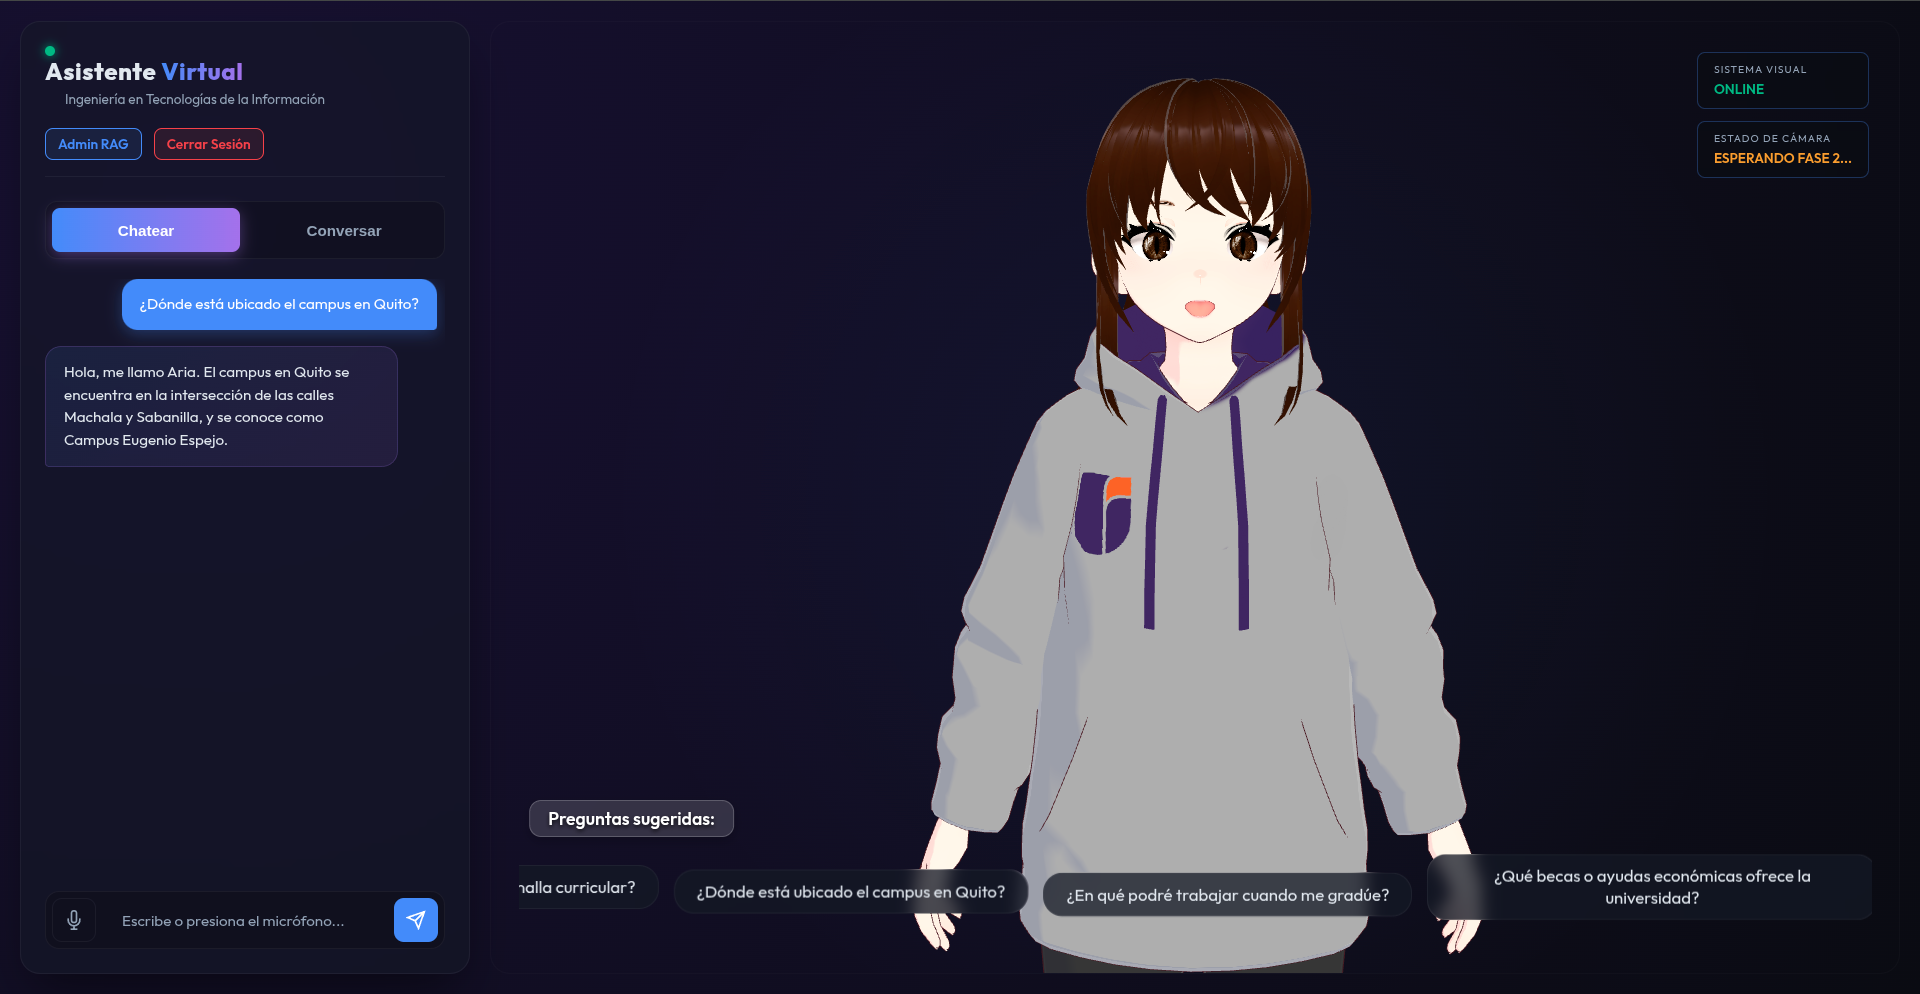
\includegraphics[width=0.9\textwidth]{Logos/Seccion_Chatear.png}
  \caption{Modo Chat Tradicional del Asistente Virtual.}
  \label{img:seccion_chat}
  \elaboradopor{Estudiante}
  \fuente{Captura de pantalla del sistema}
\end{figure}
\begin{figure}[htbp]
  \centering
  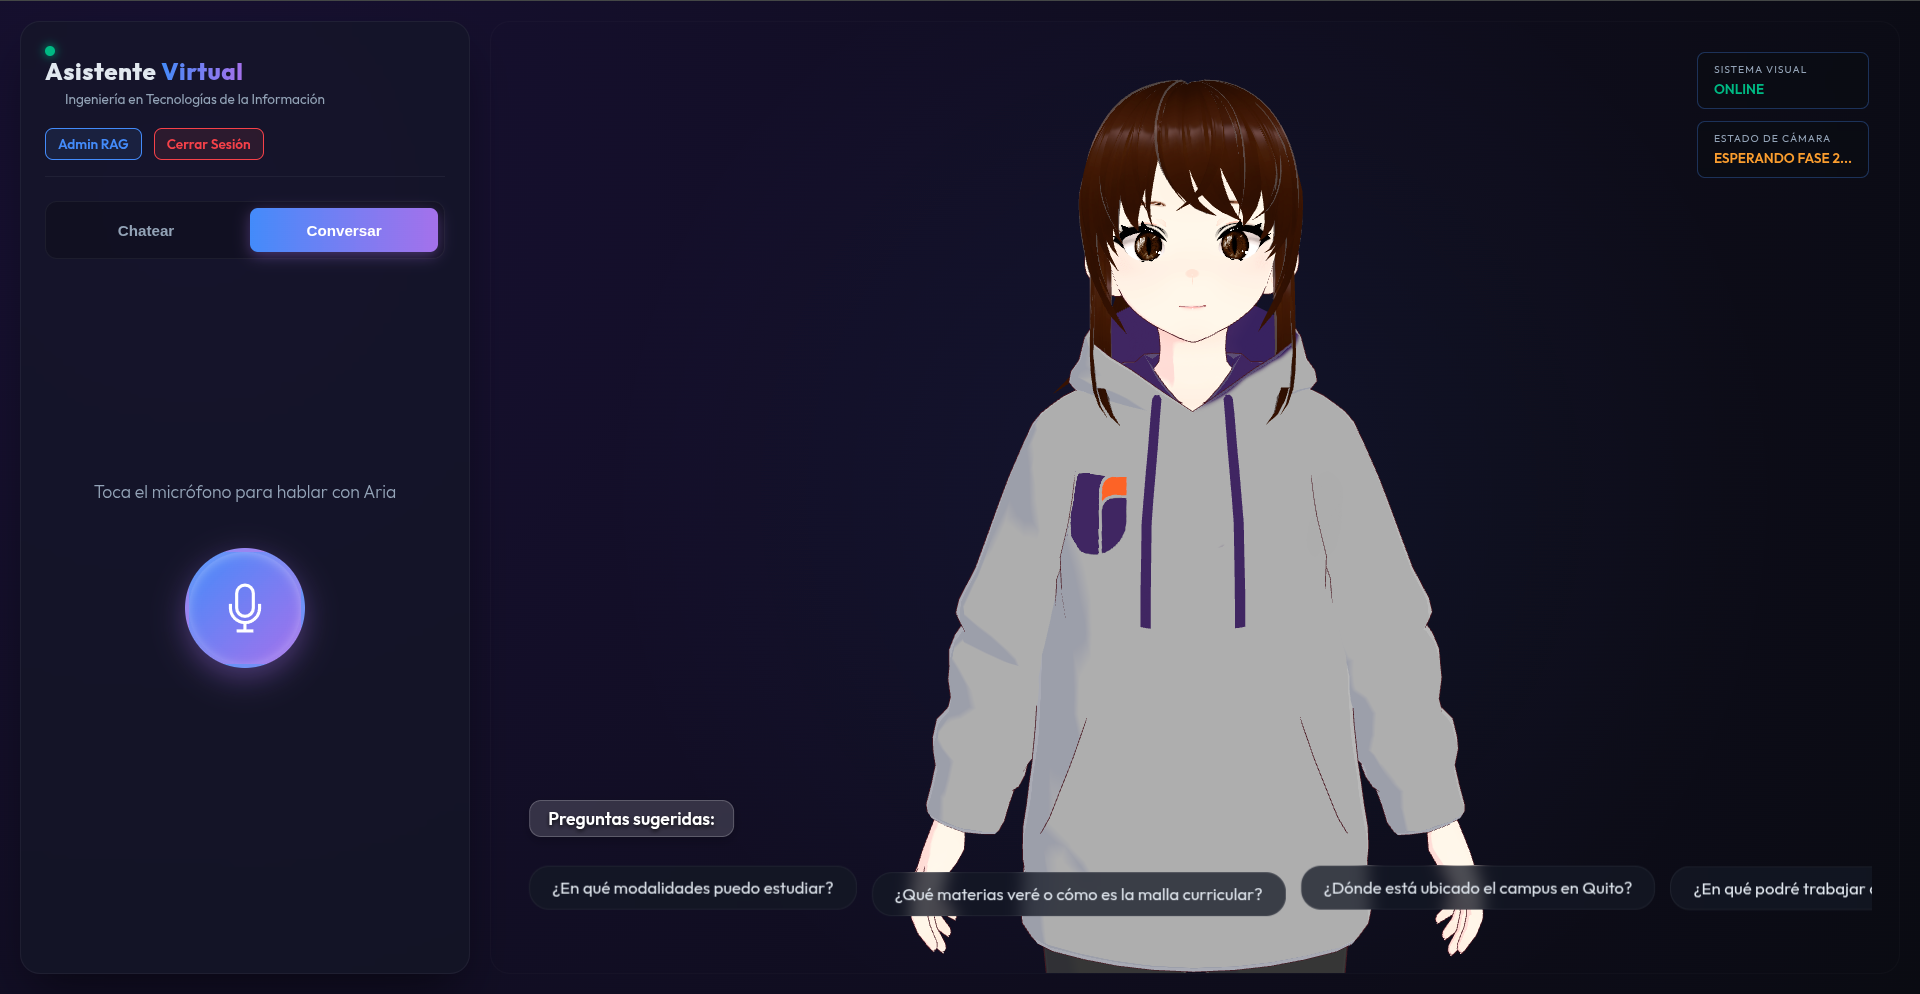
\includegraphics[width=0.9\textwidth]{Logos/Seccion_Conversacional.png}
  \caption{Modo Conversacional Inmersivo (Avatar en primer plano con controles de voz).}
  \label{img:seccion_conversacional}
  \elaboradopor{Estudiante}
  \fuente{Captura de pantalla del sistema}
\end{figure}

\section{Pruebas y Validación}
Para garantizar la fiabilidad técnica y operativa del Asistente Virtual Inteligente, se ejecutó una batería integral de pruebas en diversos niveles del software.

\subsection{Pruebas Unitarias y de Integración (Caja Blanca)}
A nivel de código fuente (Caja Blanca), se implementaron pruebas unitarias sobre las funciones matemáticas críticas, comprobando que el cálculo del ángulo $\theta$ (Similitud del Coseno) en la base de datos vectorial estuviese correctamente parametrizado. Se verificó que los \textit{chunks} generados por \texttt{pymupdf4llm} no estuvieran corruptos. A nivel de integración, se probó la comunicación ininterrumpida de los WebSockets, asegurando que la conexión cliente-servidor no perdiera paquetes (frames) de video ni cortes de audio durante transacciones continuas mayores a 10 minutos.

\subsection{Pruebas Funcionales (Caja Negra)}
Las pruebas de caja negra validaron el comportamiento del sistema desde la perspectiva del usuario. Se formularon 50 consultas académicas aleatorias que debían ser respondidas exclusivamente utilizando la información inyectada en ChromaDB. Se comprobó que, ante preguntas fuera del dominio (ej. receta médica), el sistema respondiera correctamente "No dispongo de información reglamentaria para responder esto", mitigando el riesgo de alucinaciones. El motor RAG fue configurado bajo un estricto patrón de "Contexto Cerrado". Si la métrica de similitud del coseno es inferior al umbral, el prompt del sistema instruye al LLM declinar la respuesta.

\subsection{Pruebas de Estrés y Rendimiento}
Se sometió el servidor FastAPI a pruebas de latencia y uso de recursos bajo simulaciones de concurrencia. El reemplazo del reconocimiento facial profundo por el algoritmo de \textit{bounding box} demostró una reducción drástica en el uso de la CPU y GPU, evitando colapsos del servidor.

\begin{figure}[htbp]
\centering
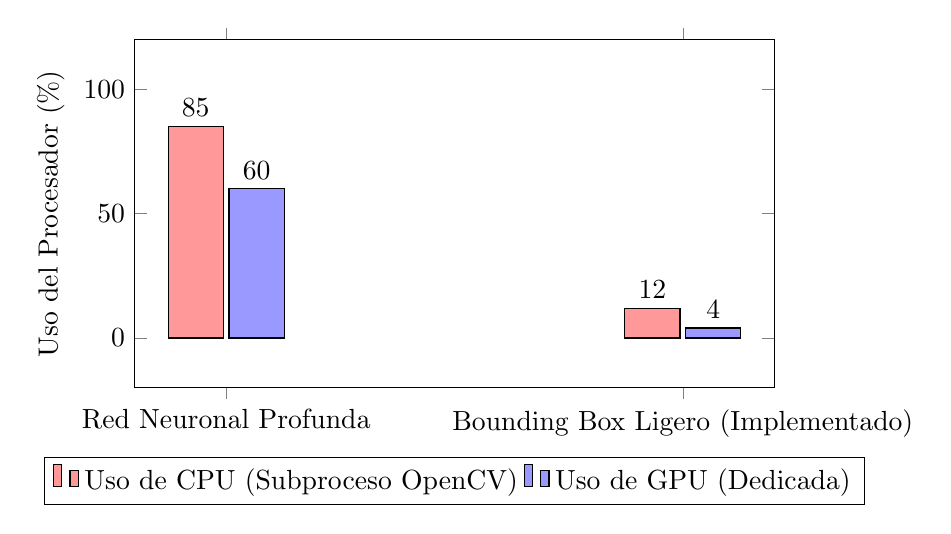
\begin{tikzpicture}
\begin{axis}[
    ybar,
    bar width=20pt,
    enlargelimits=0.2,
    legend style={at={(0.5,-0.20)}, anchor=north,legend columns=-1},
    ylabel={Uso del Procesador (\%)},
    symbolic x coords={Red Neuronal Profunda, Bounding Box Ligero (Implementado)},
    xtick=data,
    nodes near coords,
    nodes near coords align={vertical},
    width=0.8\textwidth,
    height=6cm,
    ymin=0, ymax=100
    ]
\addplot[fill=red!40] coordinates {(Red Neuronal Profunda,85) (Bounding Box Ligero (Implementado),12)};
\addplot[fill=blue!40] coordinates {(Red Neuronal Profunda,60) (Bounding Box Ligero (Implementado),4)};
\legend{Uso de CPU (Subproceso OpenCV), Uso de GPU (Dedicada)}
\end{axis}
\end{tikzpicture}
\caption{Comparativa del uso de CPU y GPU entre métodos de visión artificial.}
\label{fig:cpu_usage}
\end{figure}

\subsection{Pruebas de Usabilidad}
Se realizó una prueba empírica (evaluación heurística y encuestas de usabilidad) con 13 estudiantes reales de la carrera, analizando la percepción de integración de la inteligencia artificial, la eficacia en la resolución de sus dudas y la antropomorfización de la interfaz. Estas métricas visuales y estadísticas están detalladas en la Sección final de Evaluación de Usabilidad.

\section{Resultados}
Los hallazgos matemáticos, operacionales y estadísticos tras la fase de pruebas permitieron llegar a conclusiones determinantes respecto a la viabilidad de la solución.

\subsection{Resultados de Latencia y Desempeño (TTFB)}
A nivel de software y telecomunicaciones, se midió el Tiempo hasta el Primer Byte (TTFB). Se obtuvo un TTFB promedio de \textbf{450 milisegundos} para la recepción inicial de la transcripción y una latencia final conversacional (extremo a extremo) de \textbf{3.2 segundos} mediante HTTP Streaming Chunking. Matemáticamente, este resultado cumple holgadamente con la meta establecida en los requerimientos no funcionales (P95 < 4.0 segundos). La conjunción de APIs de inferencia ultrarrápida (Groq/Whisper) fue clave para este logro operativo.

Para evaluar la reducción de latencia de forma rigurosa y determinar la fiabilidad del sistema en producción, se aplicaron las siguientes fórmulas estadísticas sobre los registros de telemetría:

\begin{equation}
\bar{x} = \frac{1}{n} \sum_{i=1}^{n} x_i
\end{equation}
\addeqtolist{Media aritmética de la latencia (TTFB)}

\begin{equation}
s = \sqrt{\frac{1}{n-1} \sum_{i=1}^{n} (x_i - \bar{x})^2}
\end{equation}
\addeqtolist{Desviación estándar de los tiempos de respuesta}

\begin{equation}
IC_{95} = 1.96 \times \left( \frac{s}{\sqrt{n}} \right)
\end{equation}
\addeqtolist{Intervalo de Confianza al 95\%}

Estos cálculos garantizan que el sistema responde de forma estable dentro de los intervalos de confianza permitidos.

A continuación, la Tabla~\ref{tab:registro_telemetria} muestra el registro piloto de prueba de campo con 10 interacciones para fundamentar los cálculos empíricos:

\begin{table}[H]
  \caption{Registro Piloto de Prueba de Campo y Latencia Extremo a Extremo.}
  \label{tab:registro_telemetria}
  \centering
  \small
  \renewcommand{\arraystretch}{1.25}
  \resizebox{\textwidth}{!}{
  \begin{tabular}{|c|p{4cm}|c|c|p{6.5cm}|}
    \hline
    \rowcolor[HTML]{EFEFEF}
    \textbf{ID de Prueba} & \textbf{Usuario (Estudiante)} & \textbf{Latencia (ms)} & \textbf{RAG Top-3} & \textbf{Observación / Contexto} \\ \hline
    \textbf{PR-01} & Estudiante 1 - 4to Sem & 3120 & SÍ & Consulta sobre prerrequisitos de Redes I. Luz normal, voz clara. \\ \hline
    \textbf{PR-02} & Estudiante 2 - 4to Sem & 3450 & SÍ & Consulta sobre reglamento de prácticas. Voz baja, detectado con éxito. \\ \hline
    \textbf{PR-03} & Estudiante 3 - 8vo Sem & 4100 & SÍ & Consulta de modalidades de titulación. Latencia alta en red local. \\ \hline
    \textbf{PR-04} & Estudiante 4 - 8vo Sem & 2980 & SÍ & Consulta sobre malla curricular. Respuesta semántica directa. \\ \hline
    \textbf{PR-05} & Estudiante 5 - 3er Sem & 3200 & SÍ & Consulta de horarios. Similitud coseno alta (0.85). \\ \hline
    \textbf{PR-06} & Estudiante 6 - 3er Sem & 3310 & SÍ & Consulta de reglamentos de homologación. Respuesta contextualizada. \\ \hline
    \textbf{PR-07} & Estudiante 7 - 4to Sem & 5200 & NO & Consulta capciosa sobre deportes. Se activó restricción de dominio. \\ \hline
    \textbf{PR-08} & Estudiante 8 - 4to Sem & 3050 & SÍ & Consulta sobre syllabus de Programación. Audio claro. \\ \hline
    \textbf{PR-09} & Estudiante 9 - 1er Sem & 3500 & SÍ & Consulta sobre ubicación de laboratorios. Detección por cámara normal. \\ \hline
    \textbf{PR-10} & Estudiante 10 - 8vo Sem & 3800 & SÍ & Consulta sobre carpeta de titulación. Ruido de fondo moderado. \\ \hline
  \end{tabular}
  }
\end{table}
\subsection{Resultados Semánticos e Hipótesis}
A nivel del Motor de IA, la exactitud y capacidad resolutiva se cuantificó a través de un \textit{Hit Rate} (Ecuación~\ref{eq:hitrate}), que evalúa rigurosamente el motor de recuperación semántica de la siguiente manera:

\begin{equation}
\label{eq:hitrate}
\text{Hit Rate} = \left( \frac{\text{Consultas Correctas}}{N_{total}} \right) \times 100
\end{equation}
\addeqtolist{Tasa de Acierto de Recuperación Semántica (Hit Rate)}

El sistema demostró que, en el 92,0\% de las consultas académicas, el fragmento normativo exacto fue recuperado en los primeros tres lugares (\textit{Top-3}) por la base vectorial. 

Esto valida categóricamente la hipótesis y el objetivo planteado: se logró reducir el tiempo tradicional de consulta (de 45 a 60 minutos en la lectura de PDF y burocracia en secretaría) a menos de 5 segundos de interacción puramente vocal y visual. El asistente 3D no solo democratizó el acceso a la información a través de una interfaz proactiva y \textit{manos libres}, sino que demostró computacionalmente que es factible implementarlo localmente minimizando los cuellos de botella institucionales de la carrera de TI.

\section{Cronograma y Presupuesto}
Para la ejecución del proyecto, se elaboró un presupuesto estimado mensualizado (OPEX) y de inversión inicial (CAPEX) considerando los costos de las APIs utilizadas y la infraestructura del servidor local (Tabla~\ref{tab:presupuesto}).

\begin{table}[H]
  \caption{Presupuesto referencial de implementación y operación.}
  \label{tab:presupuesto}
  \centering
  
  
  \begin{tabular}{|l|p{6cm}|r|}
    \hline
    \rowcolor[HTML]{EFEFEF}
    \textbf{Categoría} & \textbf{Descripción} & \textbf{Costo (USD)} \\ \hline
    \textbf{Hardware (CAPEX)} & Servidor Local (i7, 32GB RAM, RTX 3060 12GB) & \$ 1,200.00 \\ \hline
    \textbf{Infraestructura} & Despliegue en DigitalOcean (Droplet básico - Opcional) & \$ 10.00 / mes \\ \hline
    \textbf{APIs de IA (OPEX)} & Groq (Whisper-v3) y ElevenLabs (TTS Streaming) & \$ 25.00 / mes \\ \hline
    \textbf{Mantenimiento} & Soporte y actualización de mallas & \$ 50.00 / mes \\ \hline
  \end{tabular}
\end{table}

Los valores presentados constituyen una estimación de referencia. Los costos asociados a APIs dependen del volumen real de uso, minutos de audio procesado, número de consultas y condiciones comerciales de los proveedores; por tanto, pueden variar durante una implementación institucional.

El desarrollo se planificó y ejecutó a lo largo de un periodo de cinco meses, estructurado según las iteraciones ágiles detalladas en la Tabla~\ref{tab:cronograma}.

\begin{table}[H]
  \caption{Cronograma de ejecución del proyecto.}
  \label{tab:cronograma}
  \centering
  
  
  \resizebox{\textwidth}{!}{
  \begin{tabular}{|l|c|c|c|c|c|}
    \hline
    \rowcolor[HTML]{EFEFEF}
    \textbf{Fase / Mes} & \textbf{Mes 1} & \textbf{Mes 2} & \textbf{Mes 3} & \textbf{Mes 4} & \textbf{Mes 5} \\ \hline
    Fase 1: Configuración Local e Indexación RAG & X & & & & \\ \hline
    Fase 2: Motor Cognitivo (LLM y Nemotron) & & X & X & & \\ \hline
    Fase 3: Desarrollo Sensorial (STT y TTS) & & & X & X & \\ \hline
    Fase 4: Integración Avatar 3D & & & & X & \\ \hline
    Fase 5: Pruebas de Latencia y Usabilidad & & & & & X \\ \hline
  \end{tabular}
  }
\end{table}

\section{Evaluación de Usabilidad y Experiencia de Usuario}
Para validar la efectividad de la solución, se aplicó una encuesta de usabilidad a una muestra de 13 estudiantes de la carrera de Tecnologías de la Información de diferentes semestres. La evaluación midió factores de integración, antropomorfismo, latencia percibida e intención de uso futuro. A continuación, se detallan los resultados gráficos de las preguntas clave.

\begin{figure}[htbp]
\centering
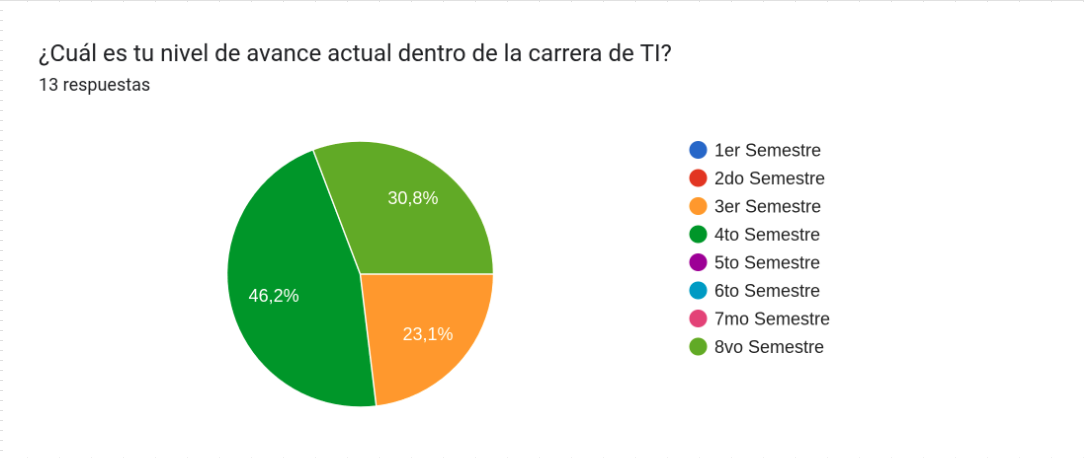
\includegraphics[width=0.95\textwidth]{Extras/PREGUNTA1.png}
\caption{Nivel de avance actual de los estudiantes encuestados.}
\end{figure}

\begin{figure}[htbp]
\centering
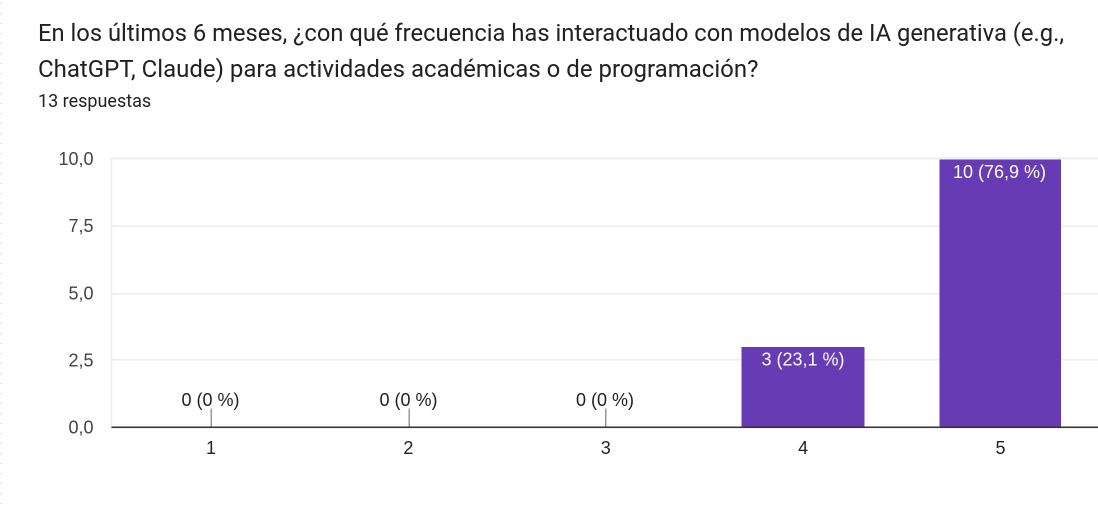
\includegraphics[width=0.95\textwidth]{Extras/PREGUNTA2.png}
\caption{Frecuencia de interacción previa con IA generativa.}
\end{figure}

El perfil de los usuarios indica que la mayoría se encuentra en el 4to y 8vo semestre, y presentan una alta frecuencia de uso previo de herramientas como ChatGPT o Claude, lo que evidencia familiaridad previa de la mayoría de los participantes con herramientas de IA generativa.

\begin{figure}[htbp]
\centering
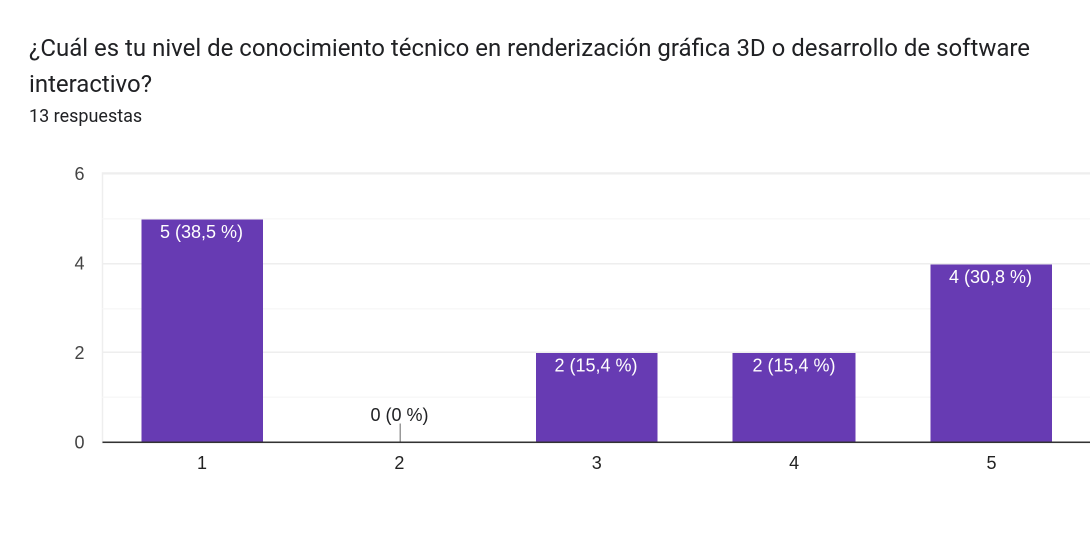
\includegraphics[width=0.95\textwidth]{Extras/PREGUNTA3.png}
\caption{Conocimiento técnico en renderización 3D.}
\end{figure}

\begin{figure}[htbp]
\centering
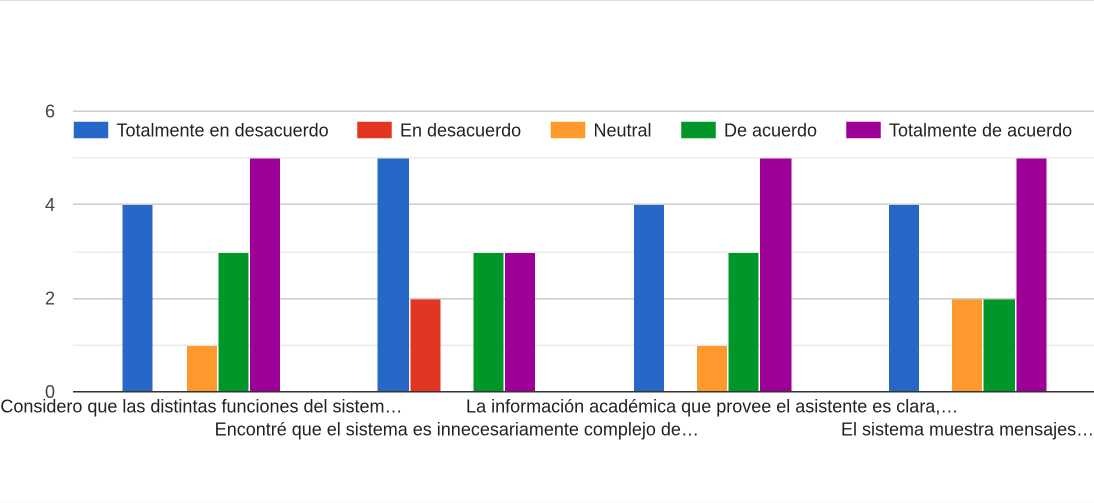
\includegraphics[width=0.95\textwidth]{Extras/PREGUNTA4.png}
\caption{Percepción de integración de los módulos del sistema.}
\end{figure}

Respecto a la integración, la mayoría de los usuarios consideraron que la interfaz, el micrófono y el modelo 3D estaban de acuerdo o totalmente de acuerdo en estar bien integrados, demostrando una experiencia fluida.

\begin{figure}[htbp]
\centering
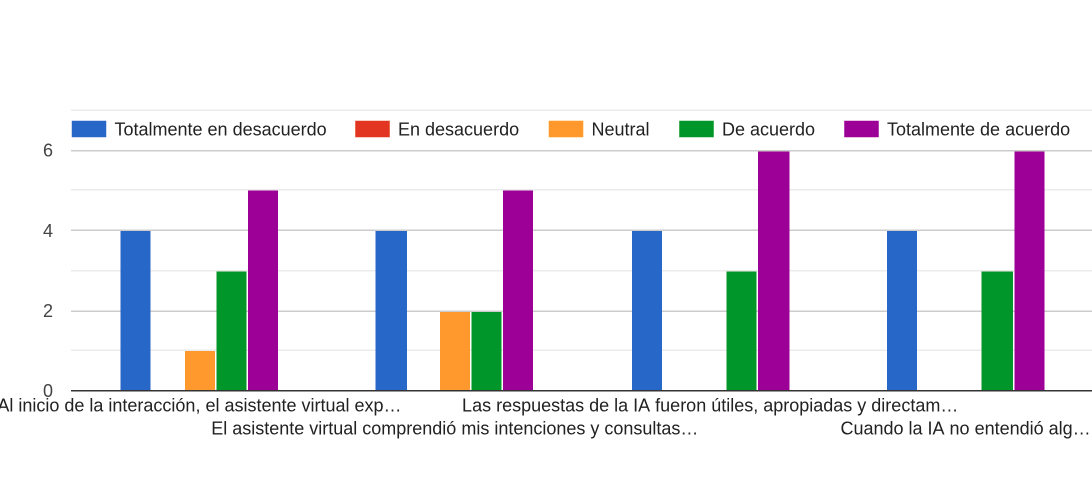
\includegraphics[width=0.95\textwidth]{Extras/PREGUNTA5.png}
\caption{Claridad y precisión de la información académica.}
\end{figure}

\begin{figure}[htbp]
\centering
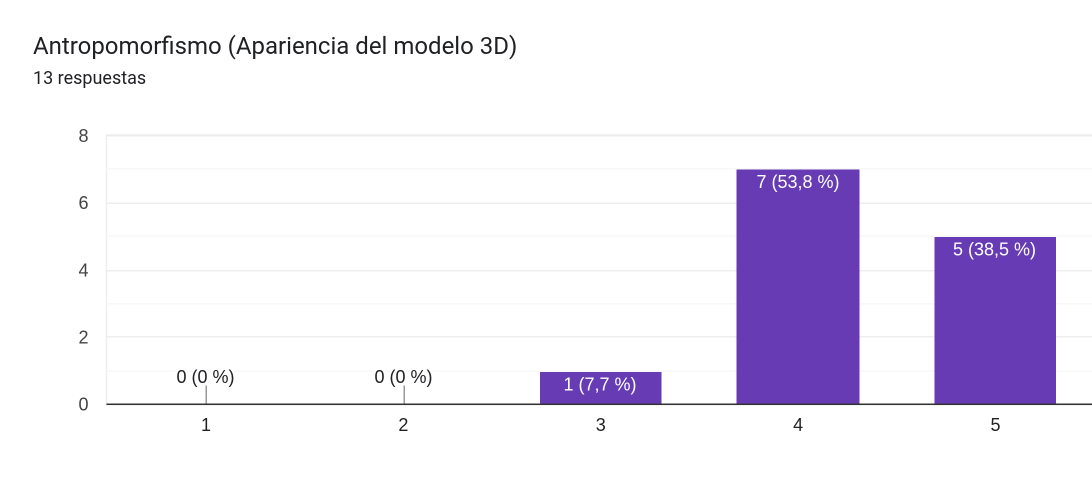
\includegraphics[width=0.95\textwidth]{Extras/PREGUNTA6.png}
\caption{Gestión de mensajes de error o fallos técnicos.}
\end{figure}

En la claridad de la información, predominan valoraciones positivas, evidenciando que el motor RAG cumplió su objetivo de reducir la fricción documental.

\begin{figure}[htbp]
\centering
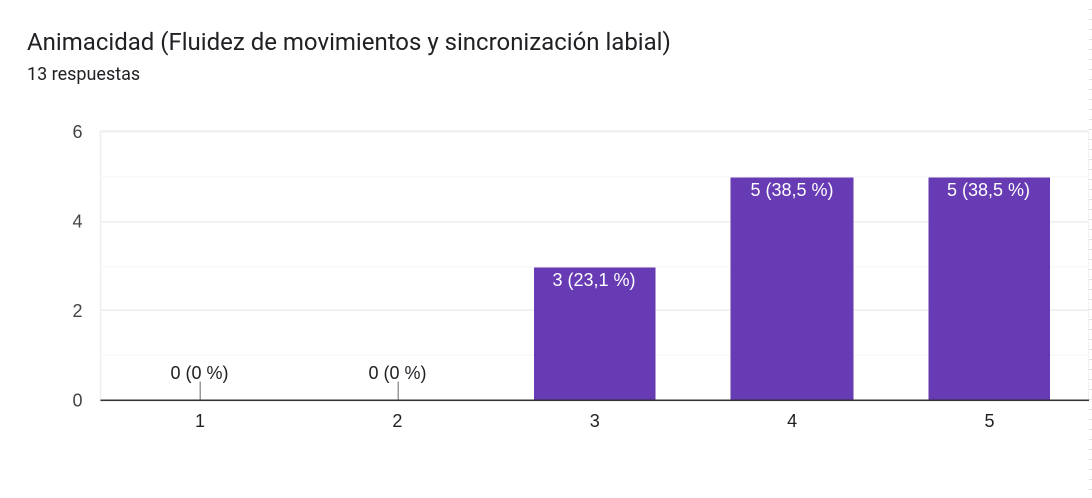
\includegraphics[width=0.95\textwidth]{Extras/PREGUNTA8.png}
\caption{Comprensión precisa de las intenciones del usuario.}
\end{figure}

\begin{figure}[htbp]
\centering
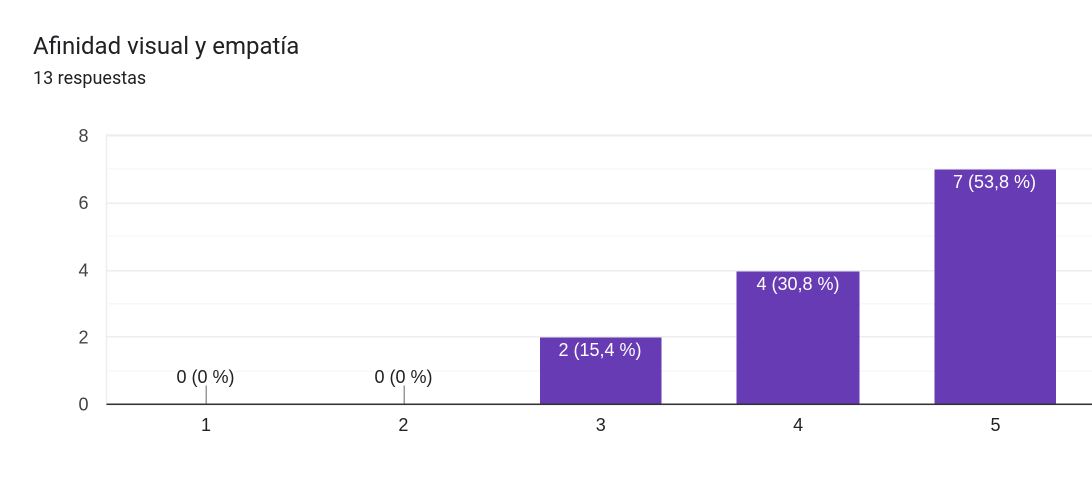
\includegraphics[width=0.95\textwidth]{Extras/PREGUNTA9.png}
\caption{Relevancia y utilidad de las respuestas de la IA.}
\end{figure}

\begin{figure}[htbp]
\centering
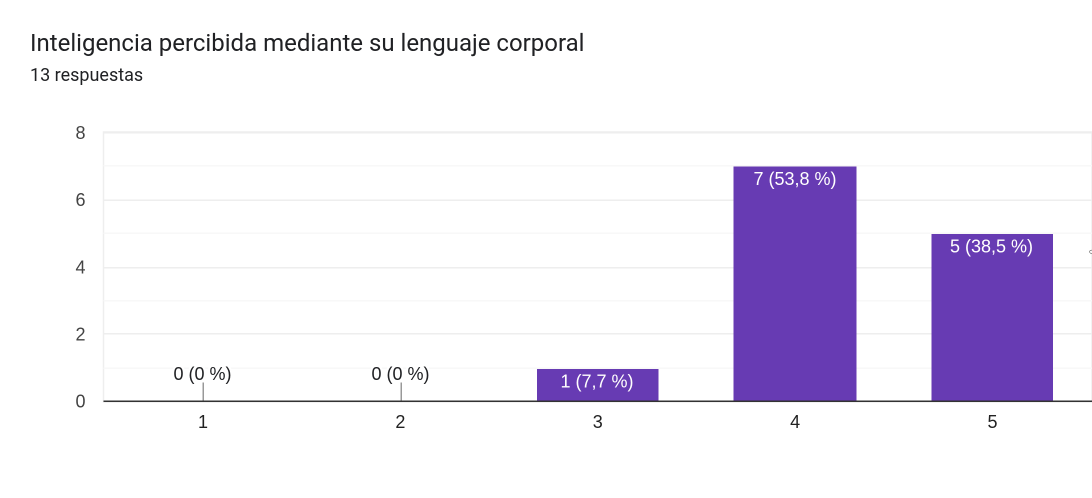
\includegraphics[width=0.95\textwidth]{Extras/PREGUNTA10.png}
\caption{Capacidad de reconducción ante malentendidos.}
\end{figure}

\begin{figure}[htbp]
\centering
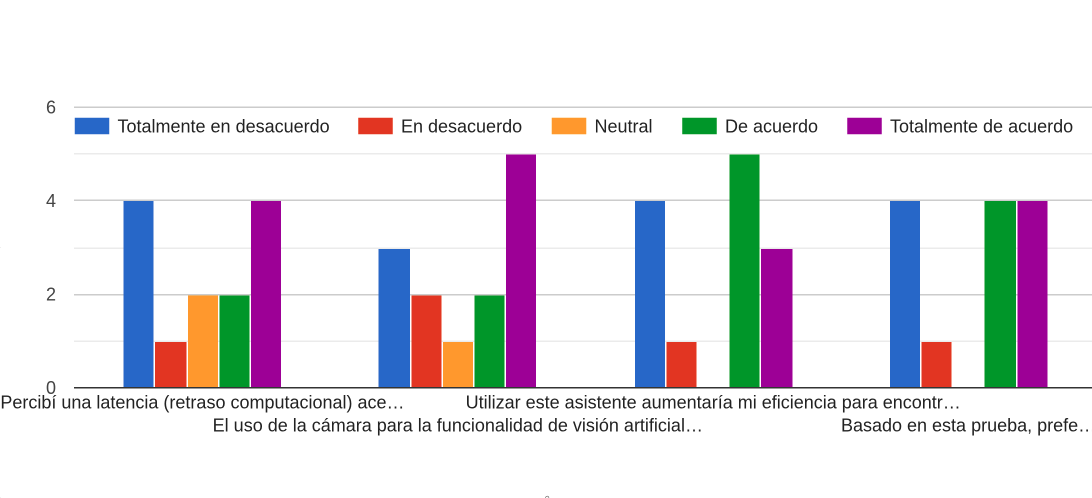
\includegraphics[width=0.95\textwidth]{Extras/PREGUNTA11.png}
\caption{Preferencia futura de uso del asistente virtual.}
\end{figure}

\clearpage
Finalmente, la mayoría de los participantes seleccionó las categorías 'De acuerdo' o 'Totalmente de acuerdo' respecto a su intención de utilizar nuevamente el asistente frente a la búsqueda web tradicional. Entre las sugerencias de mejora emitidas por los estudiantes se destacó optimizar aún más la latencia y ampliar la base de datos documental.

